\subsection{Final loss as the measure of hardness}
An alternative way of finding hard sets without any prior information is
to simply rank training examples based on their final loss values.
Here, we analyze that and compare with our approach.

One issue with picking examples with loss is that we need to find a threshold value for loss and 
keep only examples with loss value smaller that the threshold.
In this graph we show that the optimum value of this threshold is 
close to the size of forgettables.


\begin{figure}
    \centering
    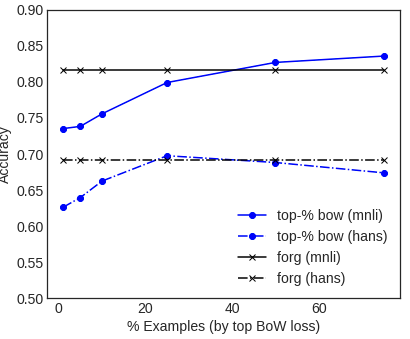
\includegraphics[width=0.5\textwidth]{figures/loss_vs_forg.png}
    \caption{Accuracy on MNLI and HANS when the finetuning set is picked
    from examples in forgettables or in a range of percentages of examples with highest loss.}
    \label{fig:loss_forg}
\end{figure}



